\section{Приложения}

\subsection{Примеры задач} \label{examples}

\begin{itemize}
    \item Задача 1:
    \[
    \begin{cases}
        y'' + y = -x; \\
        y(0) = 0, \quad y(1) = 0; \\
        y(x) = \dfrac{\sin x}{\sin 1} - x
    \end{cases}
    \]\label{z1}

    \item Задача 2:
    \[
    \begin{cases}
        y'' - y = -x; \\
        y(0) = 1, \quad y(1) = e + 1; \\
        y(x) = x + e^x
    \end{cases}
    \]\label{z2}
    
    \item Задача 3:
    \[
    \begin{cases}
        y'' - \dfrac{2y}{(x+1)^2} = \dfrac{4.5}{(x+1)^{3/2}}; \\
        y(0) - 2y'(0) = 0, \quad y'(1) = -\dfrac{1}{\sqrt{2}}; \\
        y(x) = -2\sqrt{x+1}
    \end{cases}
    \]\label{z3}
\end{itemize}

\subsection{Графики решений} \label{plots}
На левом графике показаны точное решение и полученное численное решение. На правом модуль разности решений на всём отрезке.

\begin{figure}[H]
    \centering
    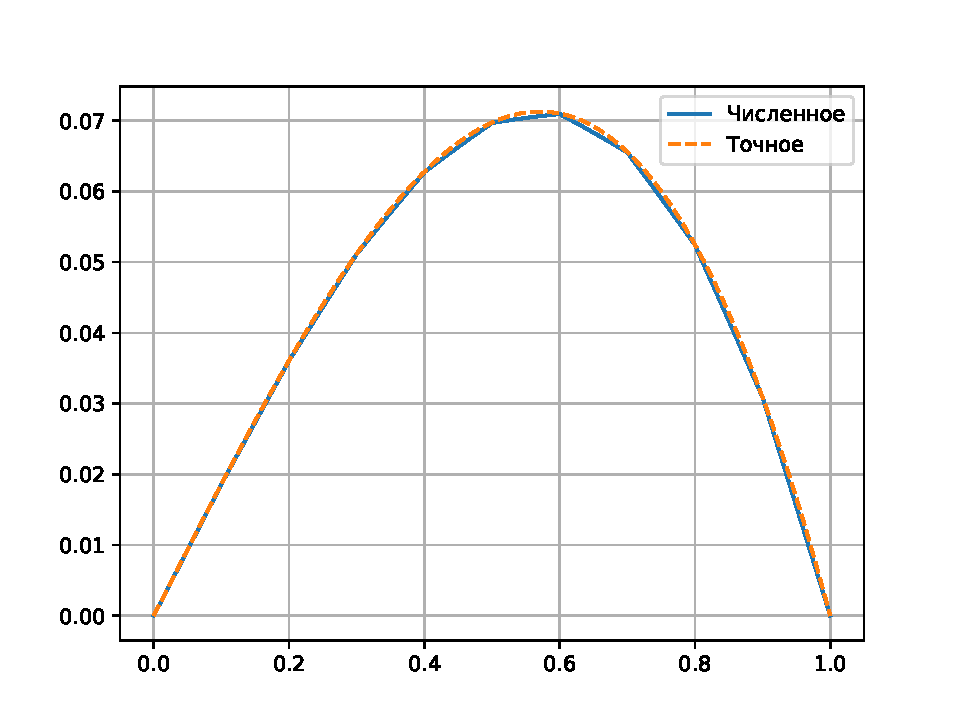
\includegraphics[width=7cm]{pictures/plot1_10.pdf}
    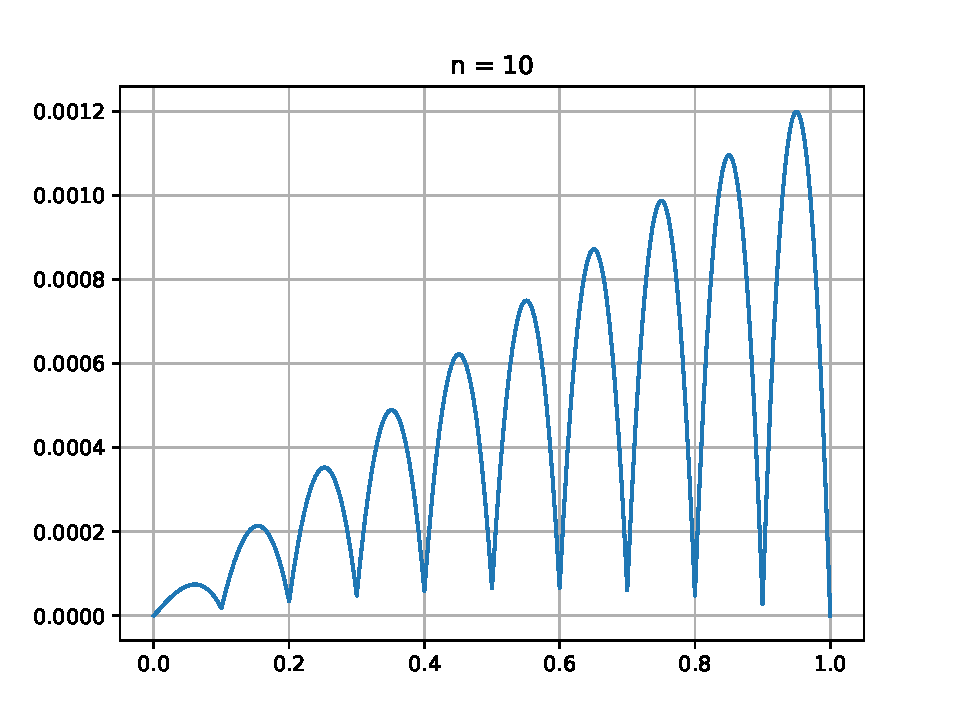
\includegraphics[width=7cm]{pictures/diff1_10.pdf}
    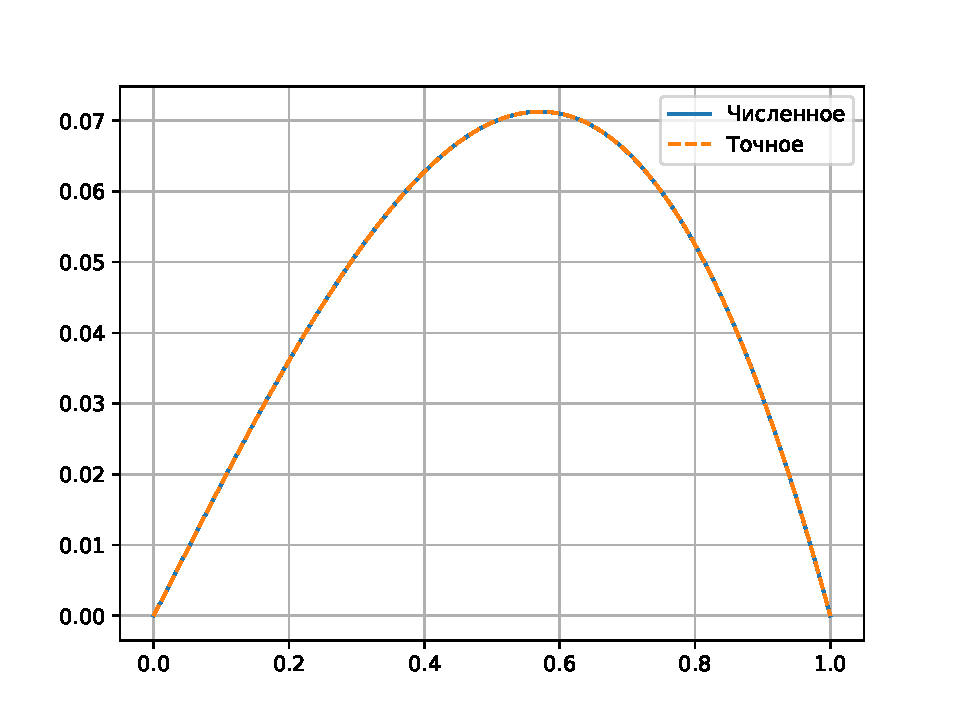
\includegraphics[width=7cm]{pictures/plot1_100.pdf}
    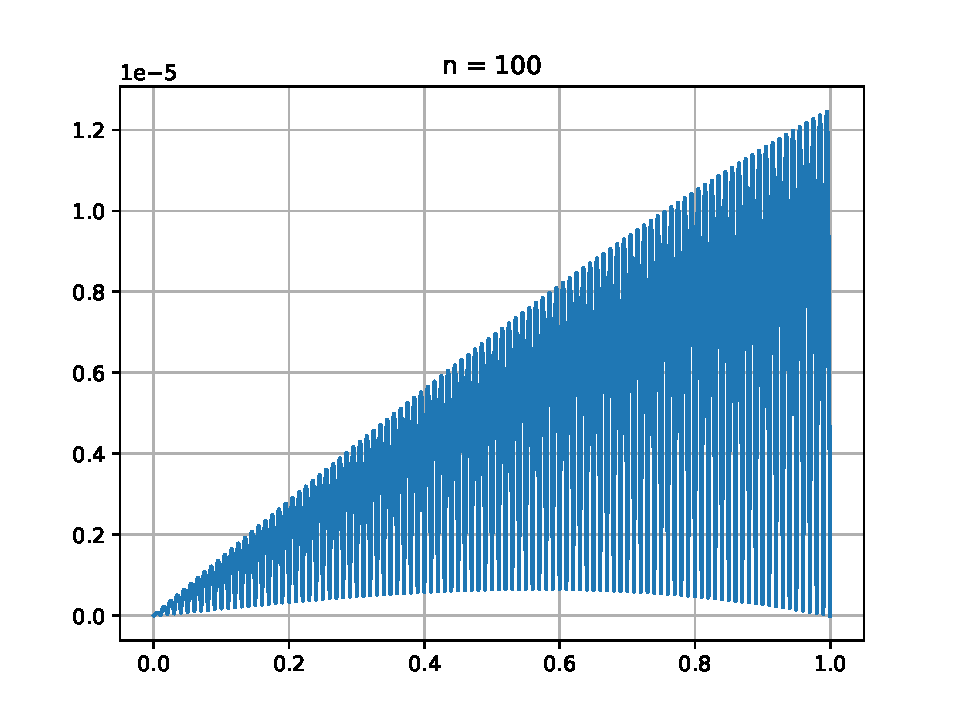
\includegraphics[width=7cm]{pictures/diff1_100.pdf}
    \caption{Задача 1 при \(N = 10\) и \(N = 100\)}\label{z1p}
\end{figure}

\begin{figure}[H]
    \centering
    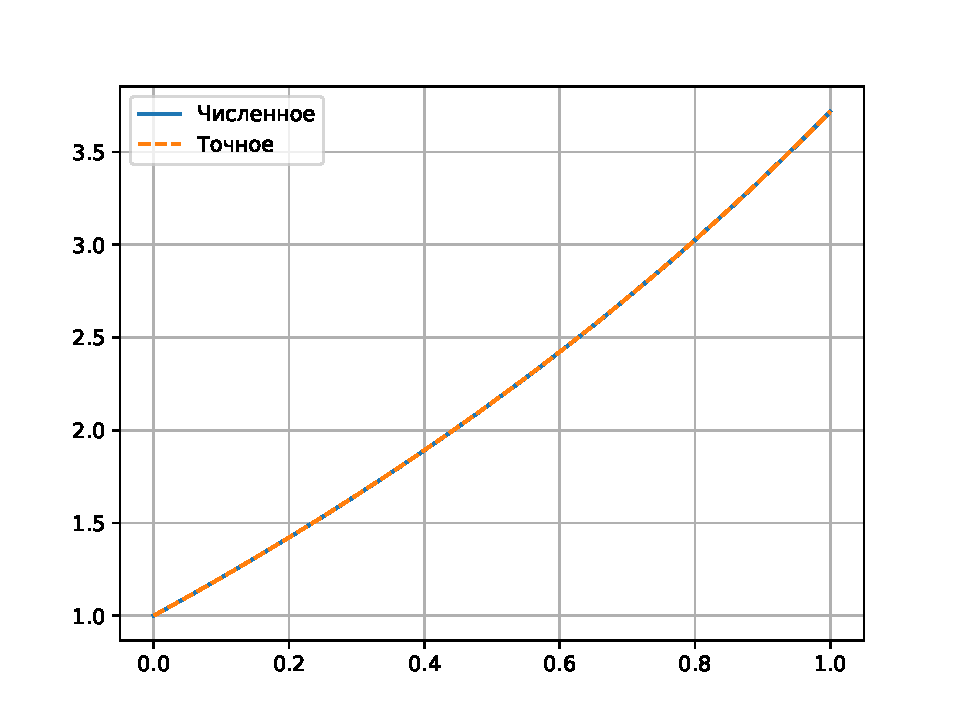
\includegraphics[width=7cm]{pictures/plot2_10.pdf}
    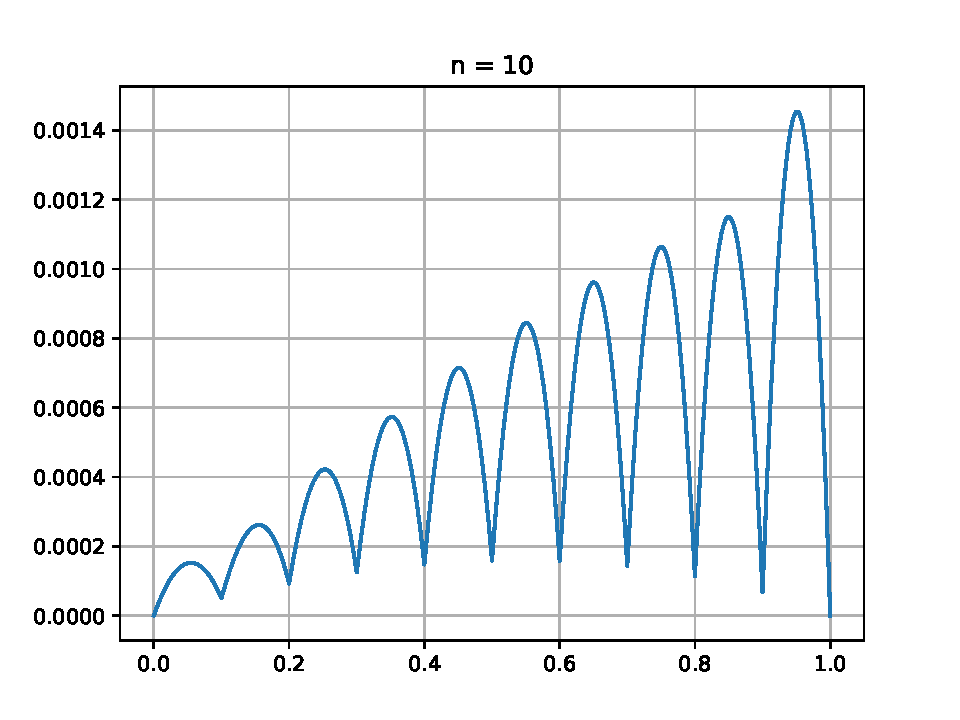
\includegraphics[width=7cm]{pictures/diff2_10.pdf}
    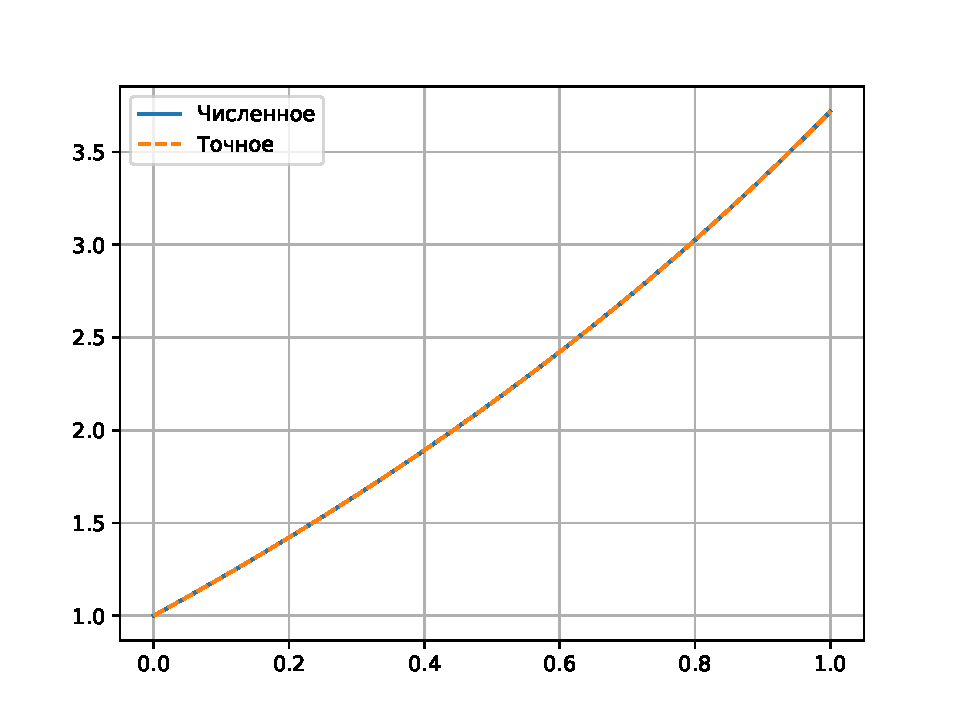
\includegraphics[width=7cm]{pictures/plot2_100.pdf}
    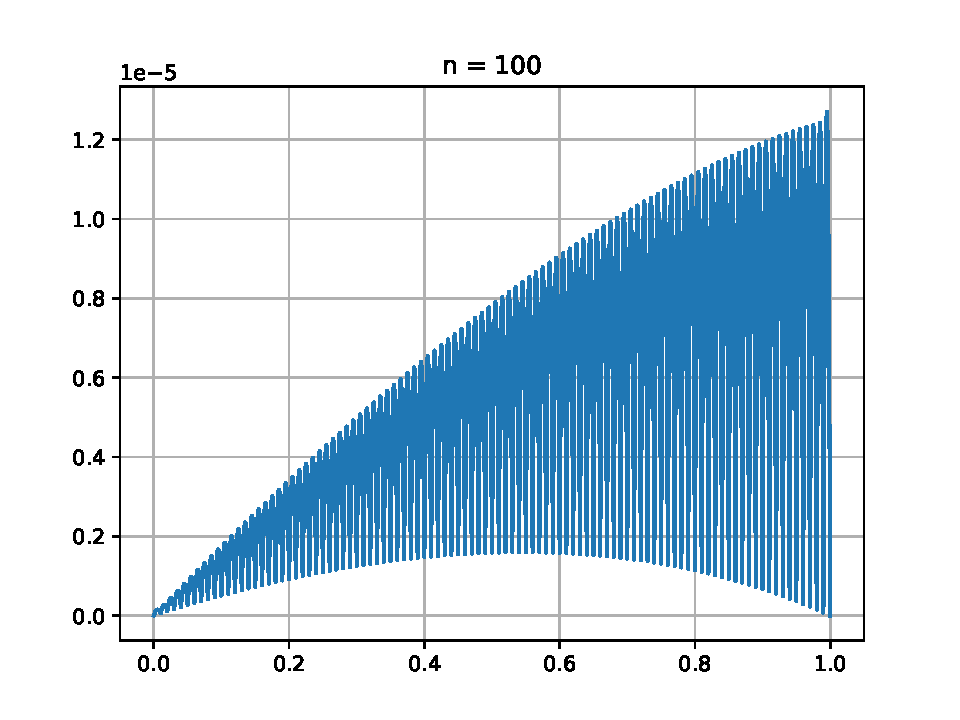
\includegraphics[width=7cm]{pictures/diff2_100.pdf}
    \caption{Задача 2 при \(N = 10\) и \(N = 100\)}\label{z2p}
\end{figure}

\begin{figure}[H]
    \centering
    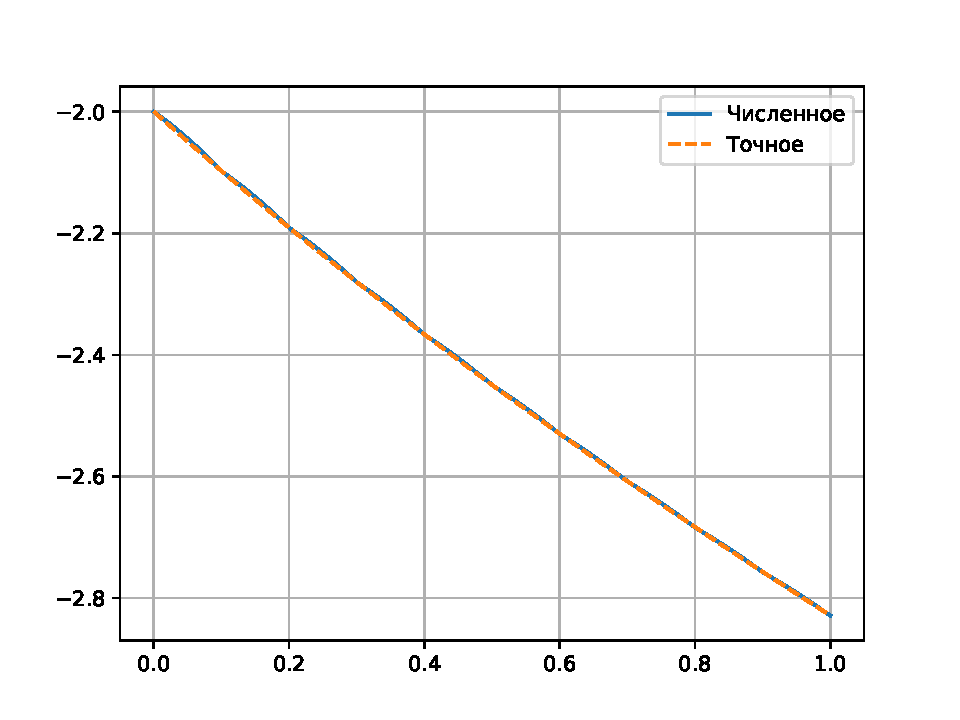
\includegraphics[width=7cm]{pictures/plot3_10.pdf}
    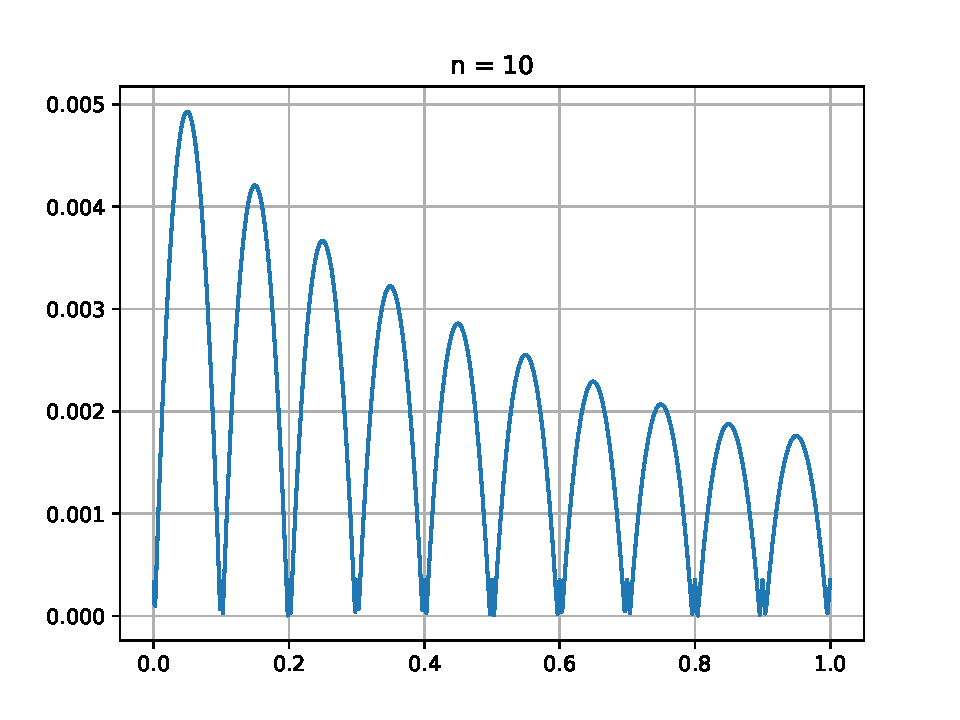
\includegraphics[width=7cm]{pictures/diff3_10.pdf}
    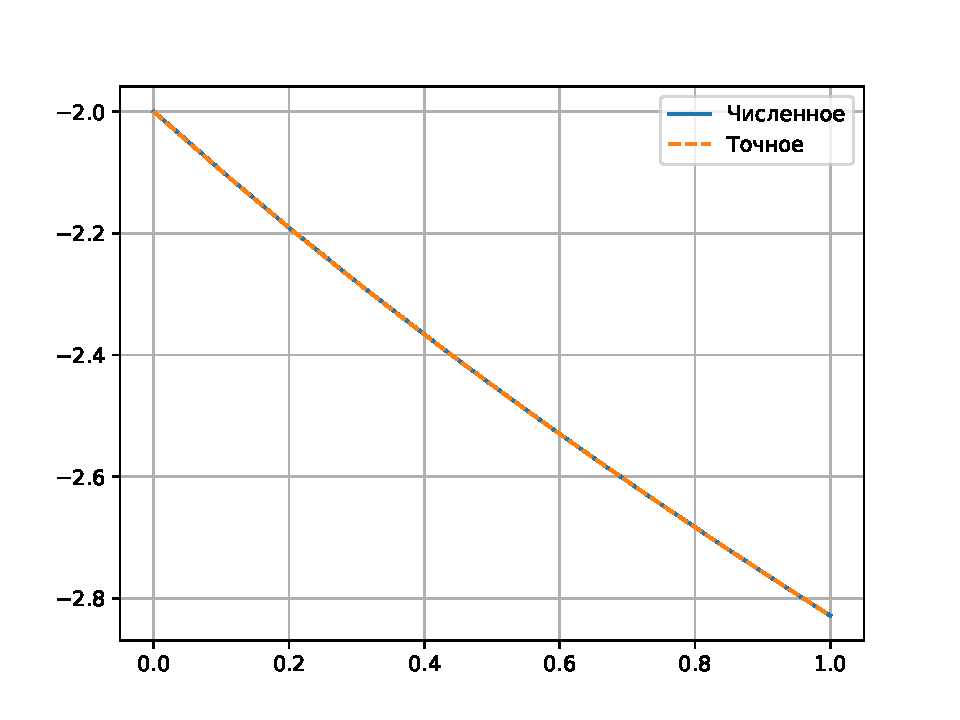
\includegraphics[width=7cm]{pictures/plot3_100.pdf}
    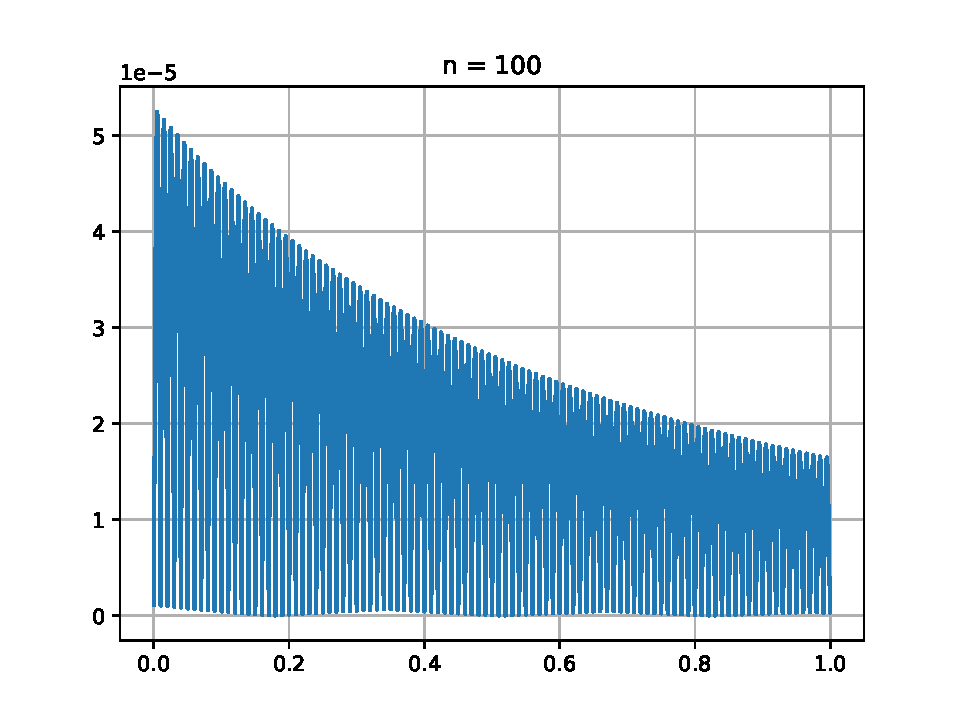
\includegraphics[width=7cm]{pictures/diff3_100.pdf}
    \caption{Задача 3 при \(N = 10\) и \(N = 100\)}\label{z3p}
\end{figure}

\subsection{Программа}

\lstinputlisting[language=Python,
            caption=Метод сплайн-коллокации.,
            captionpos=t,
            style=colored,
            basicstyle=\footnotesize\dejavu,
            frame=lines]{src/spline-c.py}